\begin{frame}

\begin{center}
\begin{tabular}{c c c}

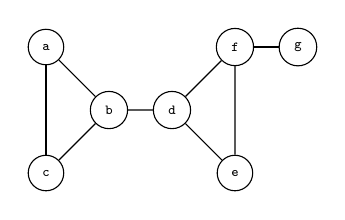
\begin{tikzpicture}[scale = 0.8]
\node[draw, circle] (a) at (0, 0) {\tiny \texttt{a}};
\node[draw, circle] (b) at (1, -1) {\tiny \texttt{b}};
\node[draw, circle] (c) at (0, -2) {\tiny \texttt{c}};
\node[draw, circle] (d) at (2, -1) {\tiny \texttt{d}};
\node[draw, circle] (f) at (3, 0) {\tiny \texttt{f}};
\node[draw, circle] (e) at (3, -2) {\tiny \texttt{e}};
\node[draw, circle] (g) at (4, 0) {\tiny \texttt{g}};

\draw (a) -- (b);
\draw (a) -- (c);
\draw (c) -- (b);
\draw (b) -- (d);
\draw (f) -- (d);
\draw (d) -- (e);
\draw (f) -- (e);
\draw (f) -- (g);

\end{tikzpicture}

&

\quad

&

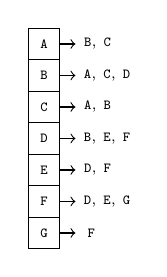
\begin{tikzpicture}[scale = 0.4]
\draw (0, -1) grid (1, 6);
\node at (0.5, -0.5) {\tiny \texttt{G}};
\node at (0.5, 0.5) {\tiny \texttt{F}};
\node at (0.5, 1.5) {\tiny \texttt{E}};
\node at (0.5, 2.5) {\tiny \texttt{D}};
\node at (0.5, 3.5) {\tiny \texttt{C}};
\node at (0.5, 4.5) {\tiny \texttt{B}};
\node at (0.5, 5.5) {\tiny \texttt{A}};

\draw[->] (1, -0.5) -- (1.5, -0.5);
\draw[->] (1, 0.5) -- (1.5, 0.5);
\draw[->] (1, 1.5) -- (1.5, 1.5);
\draw[->] (1, 2.5) -- (1.5, 2.5);
\draw[->] (1, 3.5) -- (1.5, 3.5);
\draw[->] (1, 4.5) -- (1.5, 4.5);
\draw[->] (1, 5.5) -- (1.5, 5.5);


\node at (2.2, 5.5) {\tiny \texttt{B}, \texttt{C}};
\node at (2.5, 4.5) {\tiny \texttt{A}, \texttt{C}, \texttt{D}};
\node at (2.2, 3.5) {\tiny \texttt{A}, \texttt{B}};
\node at (2.5, 2.5) {\tiny \texttt{B}, \texttt{E}, \texttt{F}};
\node at (2.2, 1.5) {\tiny \texttt{D}, \texttt{F}};
\node at (2.5, 0.5) {\tiny \texttt{D}, \texttt{E}, \texttt{G}};
\node at (2, -0.5) {\tiny \texttt{F}};
\end{tikzpicture}

\end{tabular}
\end{center}

DFS execution from node \texttt{a}

\begin{center}
\begin{tikzpicture}[]


\draw[cyan, thick] (0, -2) -- (0.5, -2) node[black, anchor = west] {\footnotesize bridges};
\node[draw, circle] (a) at (0, 0) {\tiny \texttt{a}} node[above = 0.0cm of a, fill = white] {\footnotesize 0/0};

\pause

\node[draw, fill = green!50!white, circle] (a) at (0, 0) {\tiny \texttt{a}} node[above = 0.0cm of a, fill = white] {\footnotesize 0/0};

\pause

\node[draw, circle] (b) at (-1, -0.5) {\tiny \texttt{b}};
\draw[thick] (a) -- (b);


\pause

\node[draw, fill = green!50!white, circle] (b) at (-1, -0.5) {\tiny \texttt{b}} node[below = -0.0cm of b, fill = white] {\footnotesize 1/1};

\pause

\node[draw, circle] (c) at (-2, -1) {\tiny \texttt{c}} node[left = 0.0cm of c, fill = white] {\footnotesize 2/2};
\draw[thick] (b) -- (c);

\pause 

\node[draw, fill = green!50!white, circle] (c) at (-2, -1) {\tiny \texttt{c}} node[left = 0.0cm of c, fill = white] {\footnotesize 2/2};

\pause

\draw[dashed, red] (c) edge[bend left] (a);
\node[draw, fill = green!50!white, circle] (c) at (-2, -1) {\tiny \texttt{c}} node[left = 0.0cm of c, fill = white] {\footnotesize 2/0};

\pause

\node[draw, fill = red!50!white, circle] (c) at (-2, -1) {\tiny \texttt{c}} node[left = 0.0cm of c, fill = white] {\footnotesize 2/0};
\node[draw, fill = green!50!white, circle] (b) at (-1, -0.5) {\tiny \texttt{b}} node[below = 0.0cm of b, fill = white] {\footnotesize 1/0};

\pause

\node[draw, circle] (d) at (0, -1) {\tiny \texttt{d}} node[right = 0.0cm of d, fill = white] {\footnotesize 3/3};
\draw[thick] (b) -- (d);

\pause

\node[draw, fill = green!50!white, circle] (d) at (0, -1) {\tiny \texttt{d}} node[right = 0.0cm of d, fill = white] {\footnotesize 3/3};

\pause

\node[draw, fill = green!50!white, circle] (e) at (-1, -1.5) {\tiny \texttt{e}} node[below = 0.0cm of e, fill = white] {\footnotesize 4/4};
\draw[thick] (d) -- (e);

\pause

\node[draw, fill = green!50!white, circle] (f) at (-2, -2) {\tiny \texttt{f}} node[left = 0.0cm of f, fill = white] {\footnotesize 5/5};
\draw[thick] (f) -- (e);

\pause

\node[draw, fill = green!50!white, circle] (f) at (-2, -2) {\tiny \texttt{f}} node[left = 0.0cm of f, fill = white] {\footnotesize 5/3};
\draw[dashed, red] (f) edge[bend left] (d);

\pause

\node[draw, fill = green!50!white, circle] (g) at (-1, -2.5) {\tiny \texttt{g}} node[below = 0.0cm of g, fill = white] {\footnotesize 6/6};
\draw[thick] (f) -- (g);

\pause

\node[draw, fill = red!50!white, circle] (g) at (-1, -2.5) {\tiny \texttt{g}} node[below = 0.0cm of g, fill = white] {\footnotesize 6/{\color{red}6}};
\node[draw, fill = green!50!white, circle] (f) at (-2, -2) {\tiny \texttt{f}} node[left = 0.0cm of f, fill = white] {\footnotesize {\color{red}5}/3};
\draw[thick, cyan] (f) -- (g);

\pause

\node[draw, fill = red!50!white, circle] (f) at (-2, -2) {\tiny \texttt{f}};

\pause

\node[draw, fill = red!50!white, circle] (e) at (-1, -1.5) {\tiny \texttt{e}} node[below = 0.0cm of e, fill = white] {\footnotesize 4/3};

\pause

\node[draw, fill = red!50!white, circle] (d) at (0, -1) {\tiny \texttt{d}};

\pause

\node[draw, fill = red!50!white, circle] (b) at (-1, -0.5) {\tiny \texttt{b}}  node[below = -0.0cm of b, fill = white] {\footnotesize {\color{red}1}/0};
\node[draw, circle] (d) at (0, -1) {\tiny \texttt{d}} node[right = 0.0cm of d, fill = white] {\footnotesize 3/{\color{red}3}};
\draw[dashed, red] (f) edge[bend left] (d);

\draw[thick, cyan] (b) -- (d);
\pause

\node[draw, fill = red!50!white, circle] (a) at (0, 0) {\tiny \texttt{a}};

\end{tikzpicture}
\end{center}
\end{frame}
